\chapter{Introduction}

Why develop a new theoretical framework for syntax? As I see it, there are two big problems with current approaches. One is \textit{the problem of atemporality}: conventional syntactic representations obscure temporal information. They depict a structure of relations that is supposedly non-temporal. For example, the representation in {\figref{fig:1:1}}(A) does not necessarily imply a temporal dimension as in (B): 

  
\begin{figure}
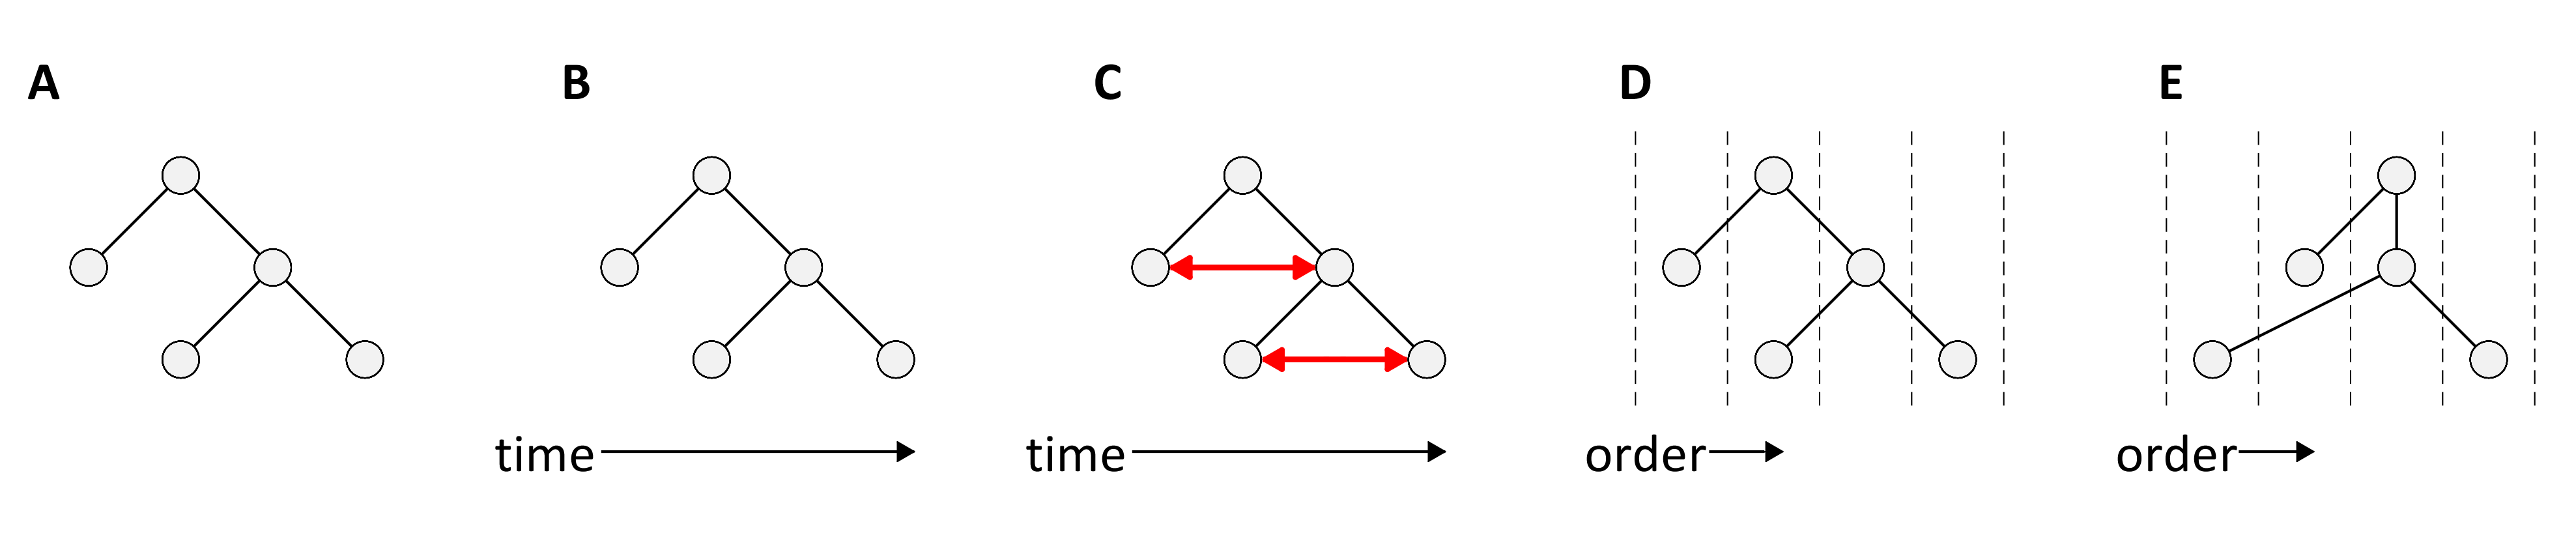
\includegraphics[width=\textwidth]{figures/Tilsen-img1.png}
\caption{Problems with time in syntactic representations.}
\label{fig:1:1}
\end{figure}
 

  If the time dimension in (B) made sense, we could draw inferences from horizontal distances between units: two horizontally equidistant units as in (C) would be equidistant in time. This is never the intent of such representations, and in many uses, the horizontal dimension does not even represent order, i.e. discretized time. Hence (D) is equivalent to (E). Because syntactic representations lack an explicit conception of time, a separate mechanism, “\isi{linearization}”, is needed to map words to a \isi{linear order}.  However, a close analysis of \isi{linearization} reveals that temporal information is indeed present in syntactic structures, hidden in connection patterns and orientation. Syntactic structures \textit{do} provide temporal information, but do so indirectly.

  In the oscillators and energy levels framework (henceforth o/el), we bring time into the picture, but not by imposing a temporal dimension on a space which contains objects. Instead, the o/el picture evokes two conceptions of time, both of which differ from our usual, linear conception. One of these is \isi{periodic time}. Periodic time is useful because we hypothesize that a fundamental property of syntactic and conceptual systems is a capability to transiently oscillate. The transience implies that the \isi{oscillation} occurs for a brief period of time, as shown in {\figref{fig:1:2}}(A). 

  
\begin{figure}
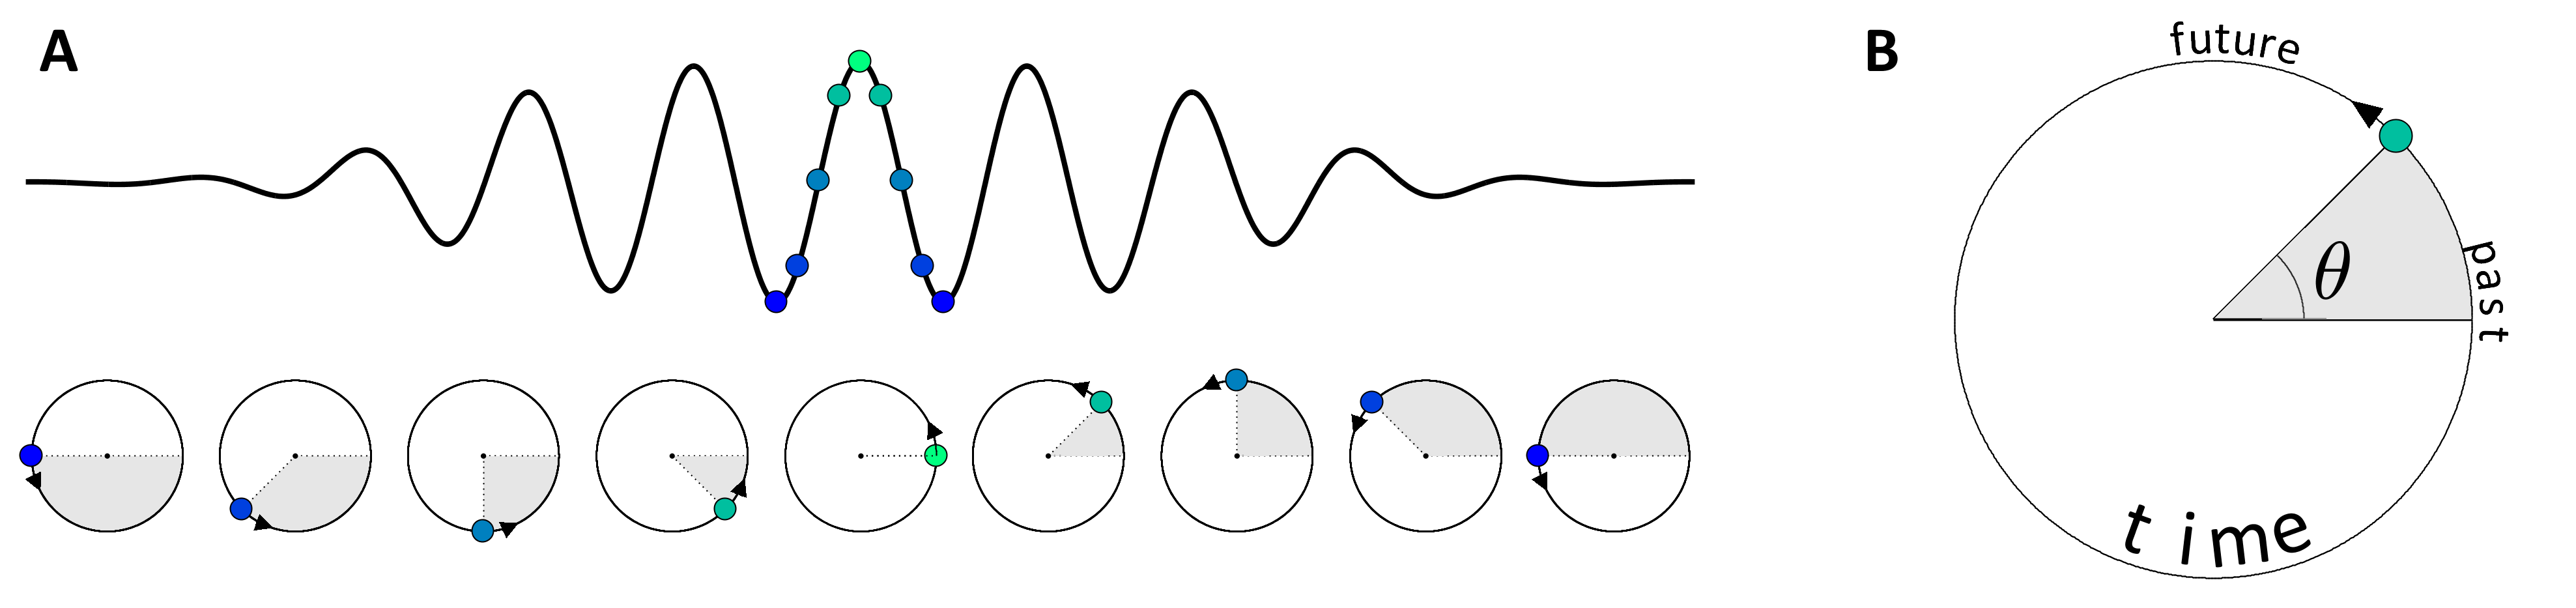
\includegraphics[width=\textwidth]{figures/Tilsen-img2.png}
\caption{Oscillations can be described with a periodic conception of time.}
\label{fig:1:2}
\end{figure}
 

  For an oscillating system, we can picture a circular axis of time as in {\figref{fig:1:2}}(B). A specific time is a particular \textit{phase angle}, θ, defined relative to a \isi{reference phase} angle. The choices of the \isi{reference phase} and angular units are arbitrary: 0°, 0 radians, or 3:00 are just as useful as 90°, π/2 radians, or 12:00. Phase angle is periodic by definition, so a phase of 360° maps to 0°. Though we are familiar with the angular mapping of time because of circular clocks, some aspects of this conception do not gel with our commonsense intuitions. For instance, \isi{periodic time} has local notions of past and future, but no global or absolute past or future. There is also an implied frequency parameter, which describes how \isi{periodic time} maps to \isi{linear time}: the period of an \isi{oscillation} (T) is the reciprocal of the frequency (\textit{f}).

  Periodic time provides a useful description of a temporal relation between a pair of oscillating systems: \textit{relative phase}, ϕ. Relative phase is the difference between the phase angles of two systems, as illustrated in {\figref{fig:1:3}}. For a pair of systems \textit{i} and \textit{j}, ϕ\textit{\textsubscript{ij}}\textsubscript{} = θ\textit{\textsubscript{i}} - θ\textit{\textsubscript{j}}. Patterns of ϕ are of fundamental importance in the o/el framework: a central proposal is that transiently stable ϕ configurations give rise to the experience of \isi{relational meaning}.  

  
\begin{figure}
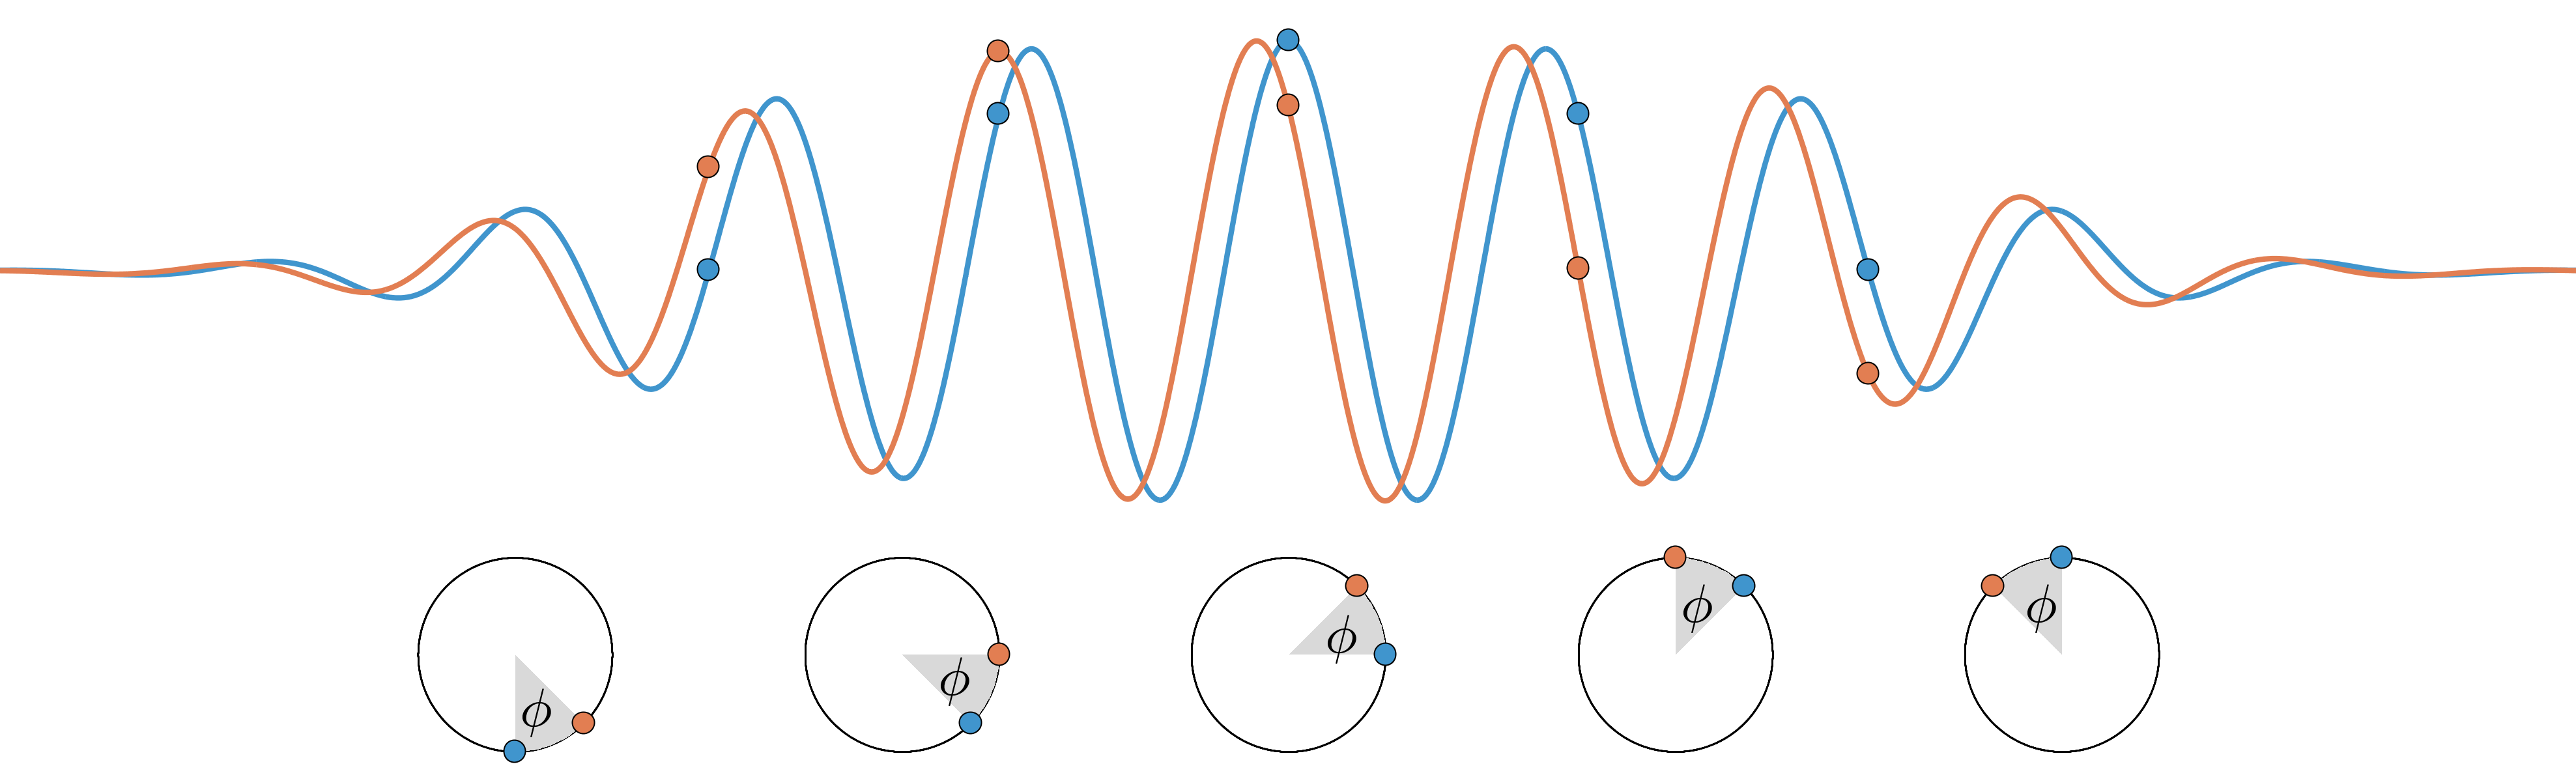
\includegraphics[width=\textwidth]{figures/Tilsen-img3.png}
\caption{Relative phase as the difference between phase angles.}
\label{fig:1:3}
\end{figure}
 

  The other conception of time in the o/el framework is discontinuous, piecewise-\isi{linear time}. Why is this useful? Let us imagine a system in which some quantity normally changes slowly or stays constant, but certain processes occasionally cause the quantity to change very abruptly. As shown in {\figref{fig:1:4}}, a continuous but highly nonlinear change of this sort can be approximated as a discontinuity when viewed on a larger scale.

  
\begin{figure}
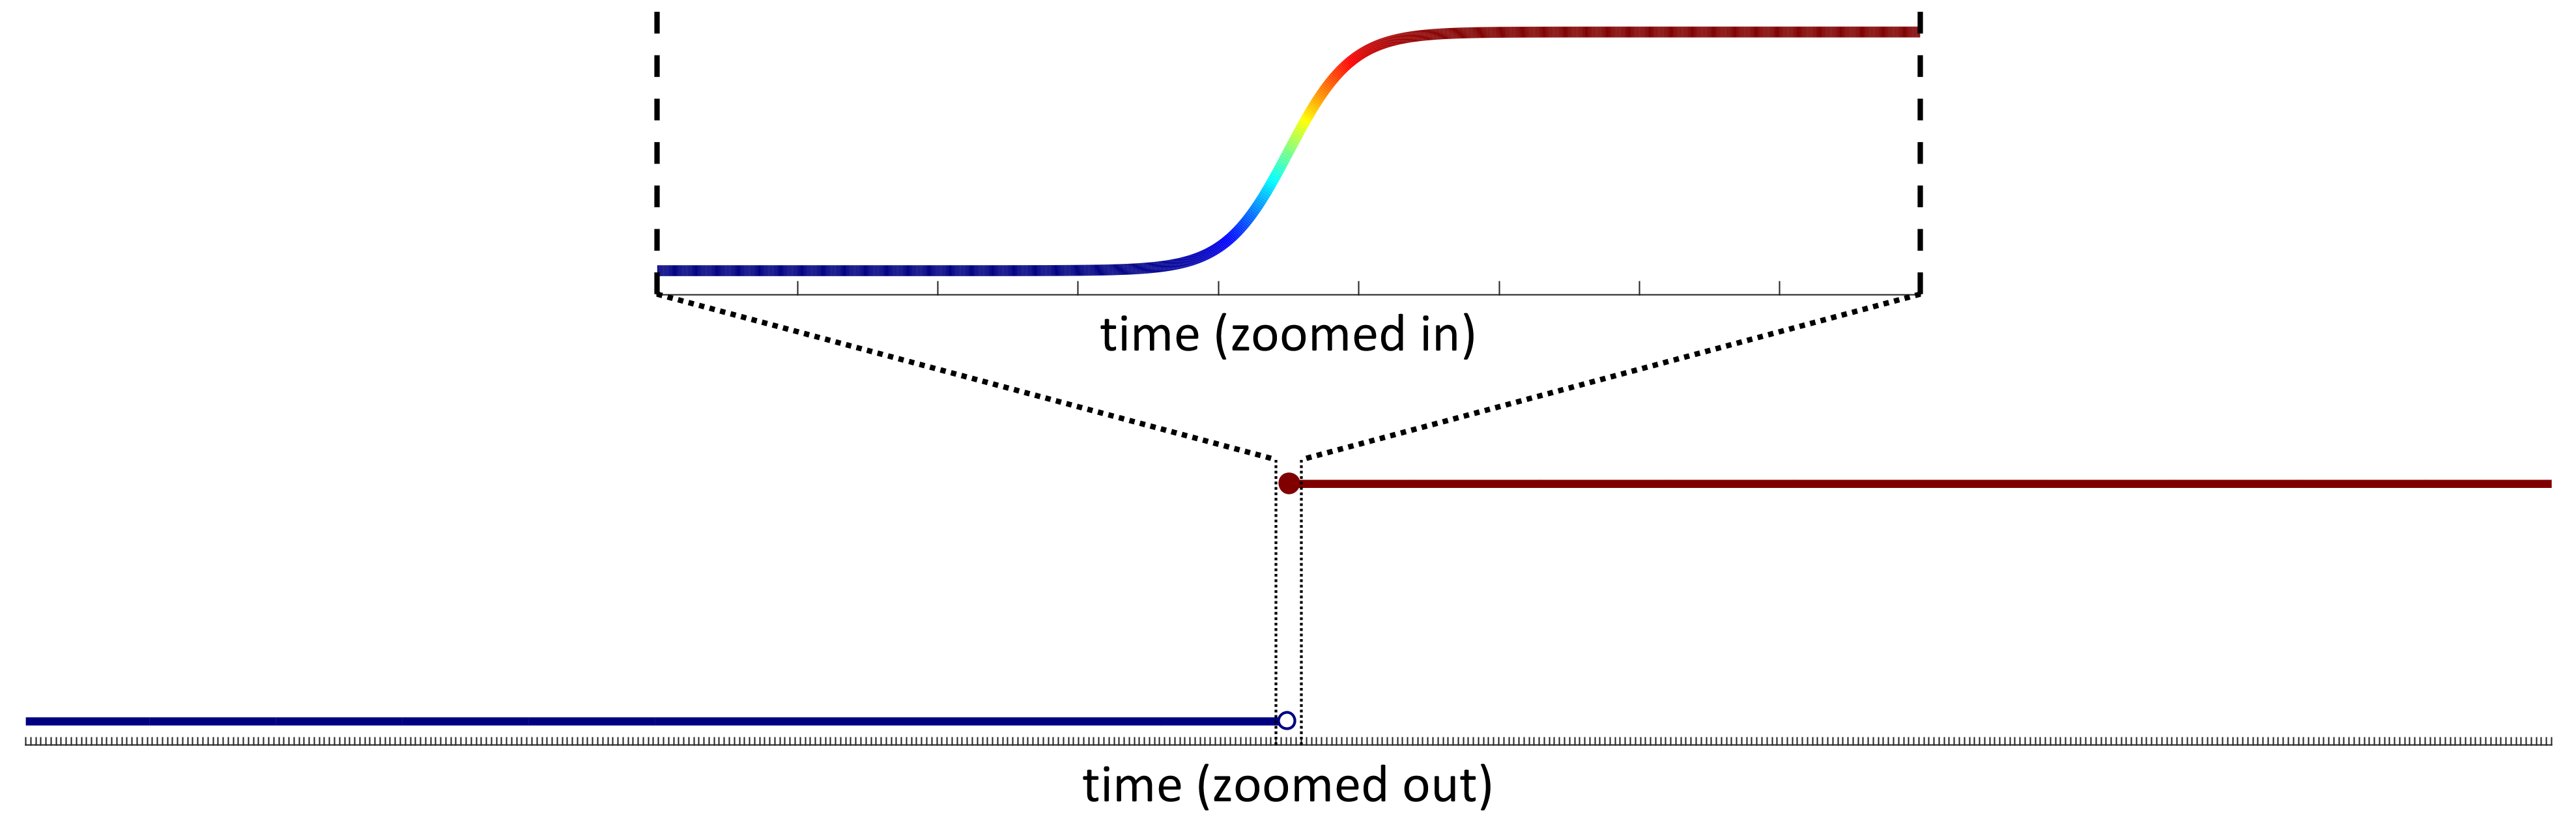
\includegraphics[width=\textwidth]{figures/Tilsen-img4.png}
\caption{Abrupt changes in a quantity can be viewed as discontinuities on a larger scale.}
\label{fig:1:4}
\end{figure}
 

  Temporal discontinuities are useful because the timescale of processes which govern the ordering of motor behaviors is smaller than the timescale on which \isi{relational meaning} experiences (i.e. ϕ patterns) remain stable. Moreover, we hypothesize a mechanism for rapid organization and reorganization of syntactic systems into hierarchically related levels of excitation, as shown in {\figref{fig:1:5}}.

  
\begin{figure}
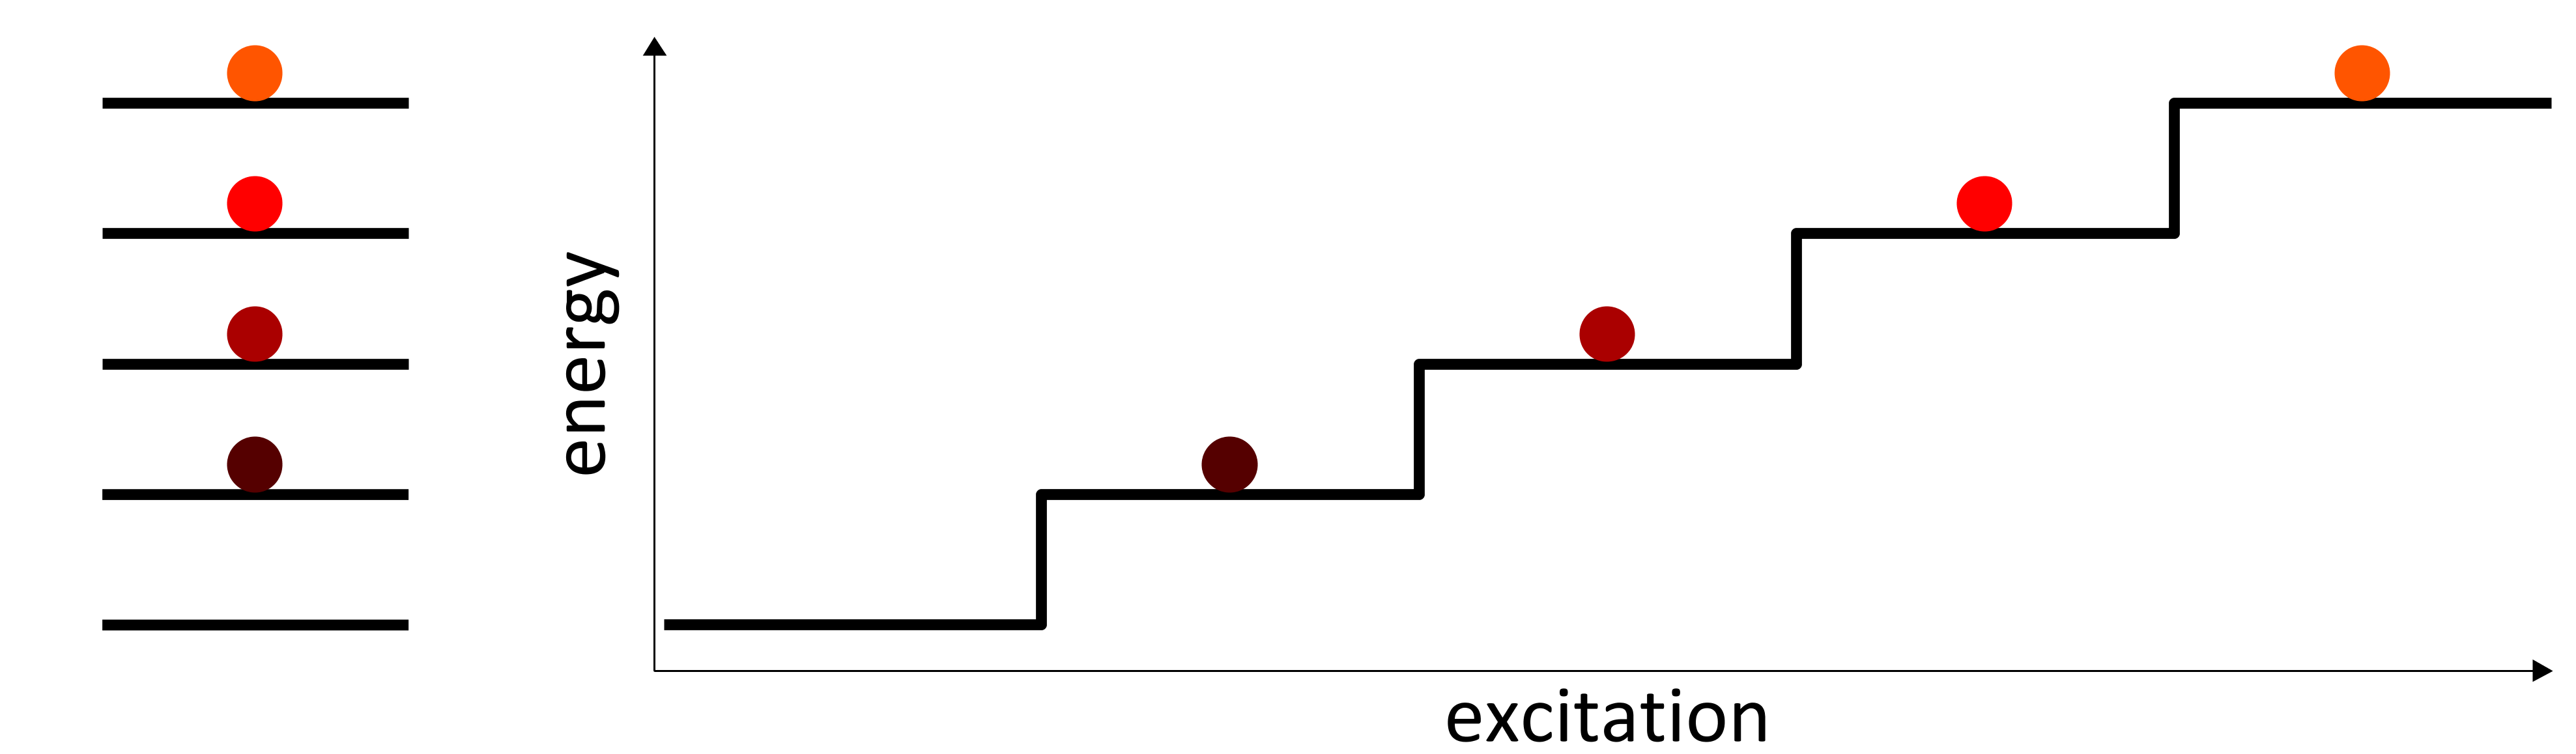
\includegraphics[width=\textwidth]{figures/Tilsen-img5.png}
\caption{Systems are organized in a hierarchy of relative excitation.}
\label{fig:1:5}
\end{figure}
 

  The production mechanism operates via iterated reorganization of the excitation hierarchy, as illustrated in {\figref{fig:1:6}}. In epoch (e\textsubscript{1}), the most highly excited system is selected and corresponding motor actions are performed. Subsequently, the selected system is demoted while other systems are promoted—a reorganization occurs, resulting in a new stable epoch, (e\textsubscript{2}). As shown in {\figref{fig:1:6}}, the reorganization process is iterated, resulting in the production of a sequence of words.

  
\begin{figure}
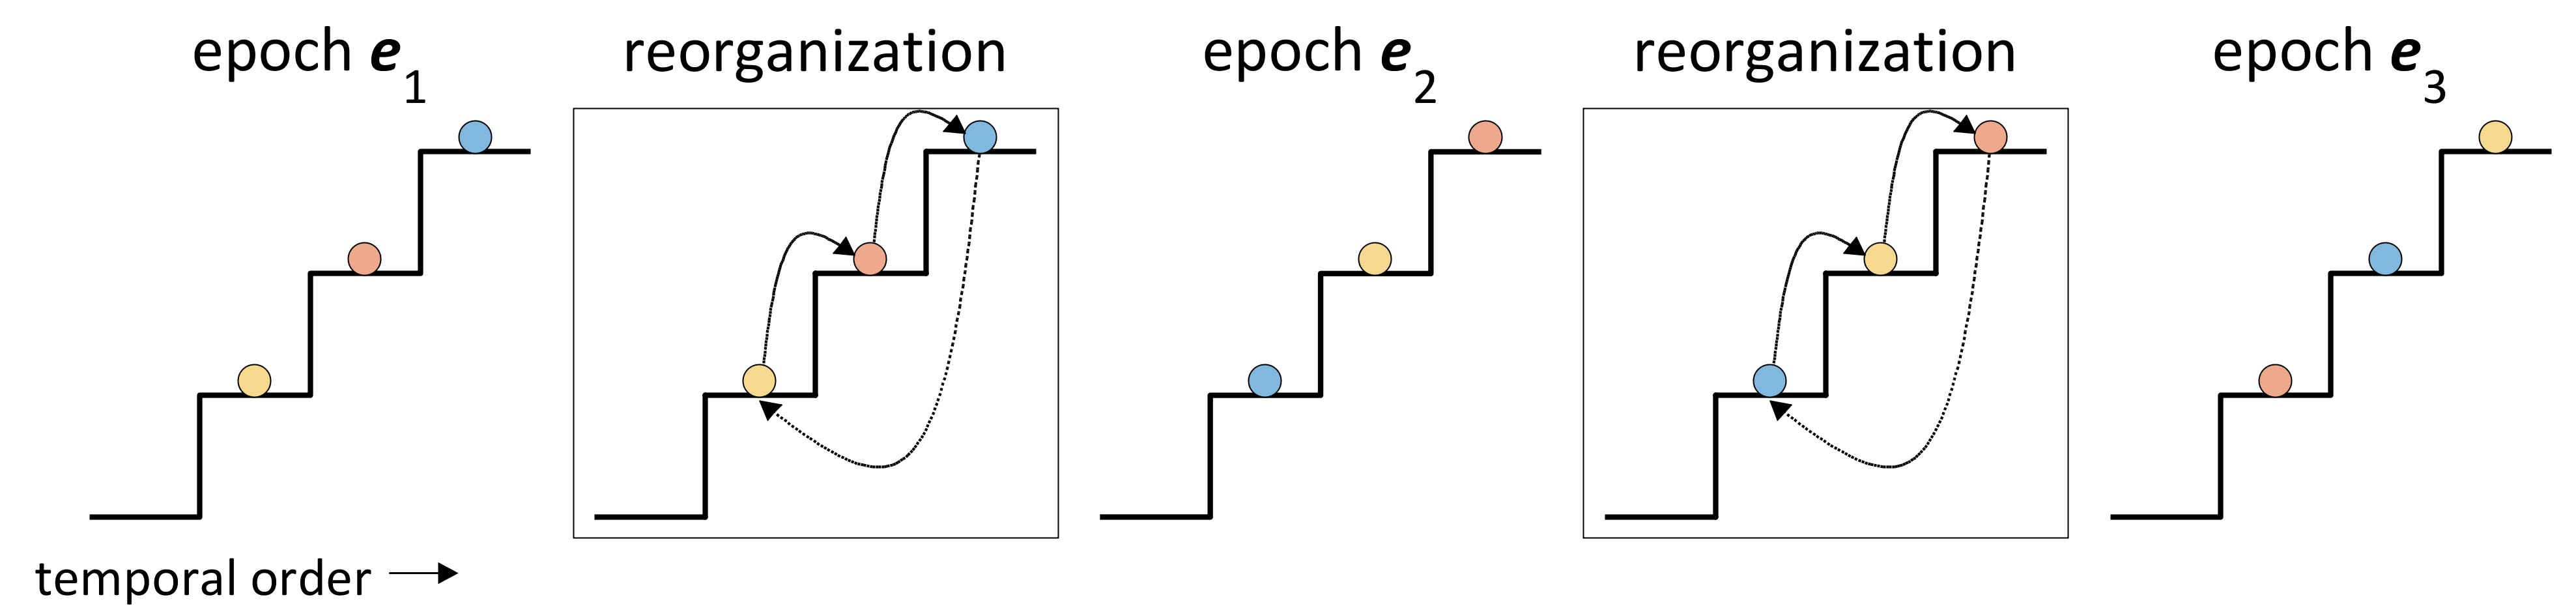
\includegraphics[width=\textwidth]{figures/Tilsen-img6.png}
\caption{Temporal order arises from iterated reorganization of the excitation hierarchy.}
\label{fig:1:6}
\end{figure}
 

  Instead of obscuring time, o/el representations are designed to facilitate reasoning about temporal patterns. The blend of temporal conceptions which is evoked by the o/el framework highlights a tension between continuity and discontinuity that underlies nearly all of our reasoning about language. Bringing this tension to the foreground helps us better understand a wide variety of syntactic phenomena in the production and interpretation of language.

The other big problem with conventional theories is the \textit{problem of multiplicity}. In syntactic trees (and many alternative representational schemas), a given type of \isi{syntactic object} (e.g. N, V, \isi{VP}, S, etc.) can be present in an arbitrary number of positions in a structure, as in {\figref{fig:1:7}}. Conventional frameworks impose no limit on the number of instantiations of a given type of object. No adverse consequences of multiplicity are expected in such approaches, even when multiplicitous objects are associated with the same word, e.g. the verb \textit{knows} in the utterance \textit{Al knows that Bo knows that Cam knows…}  

  
\begin{figure}
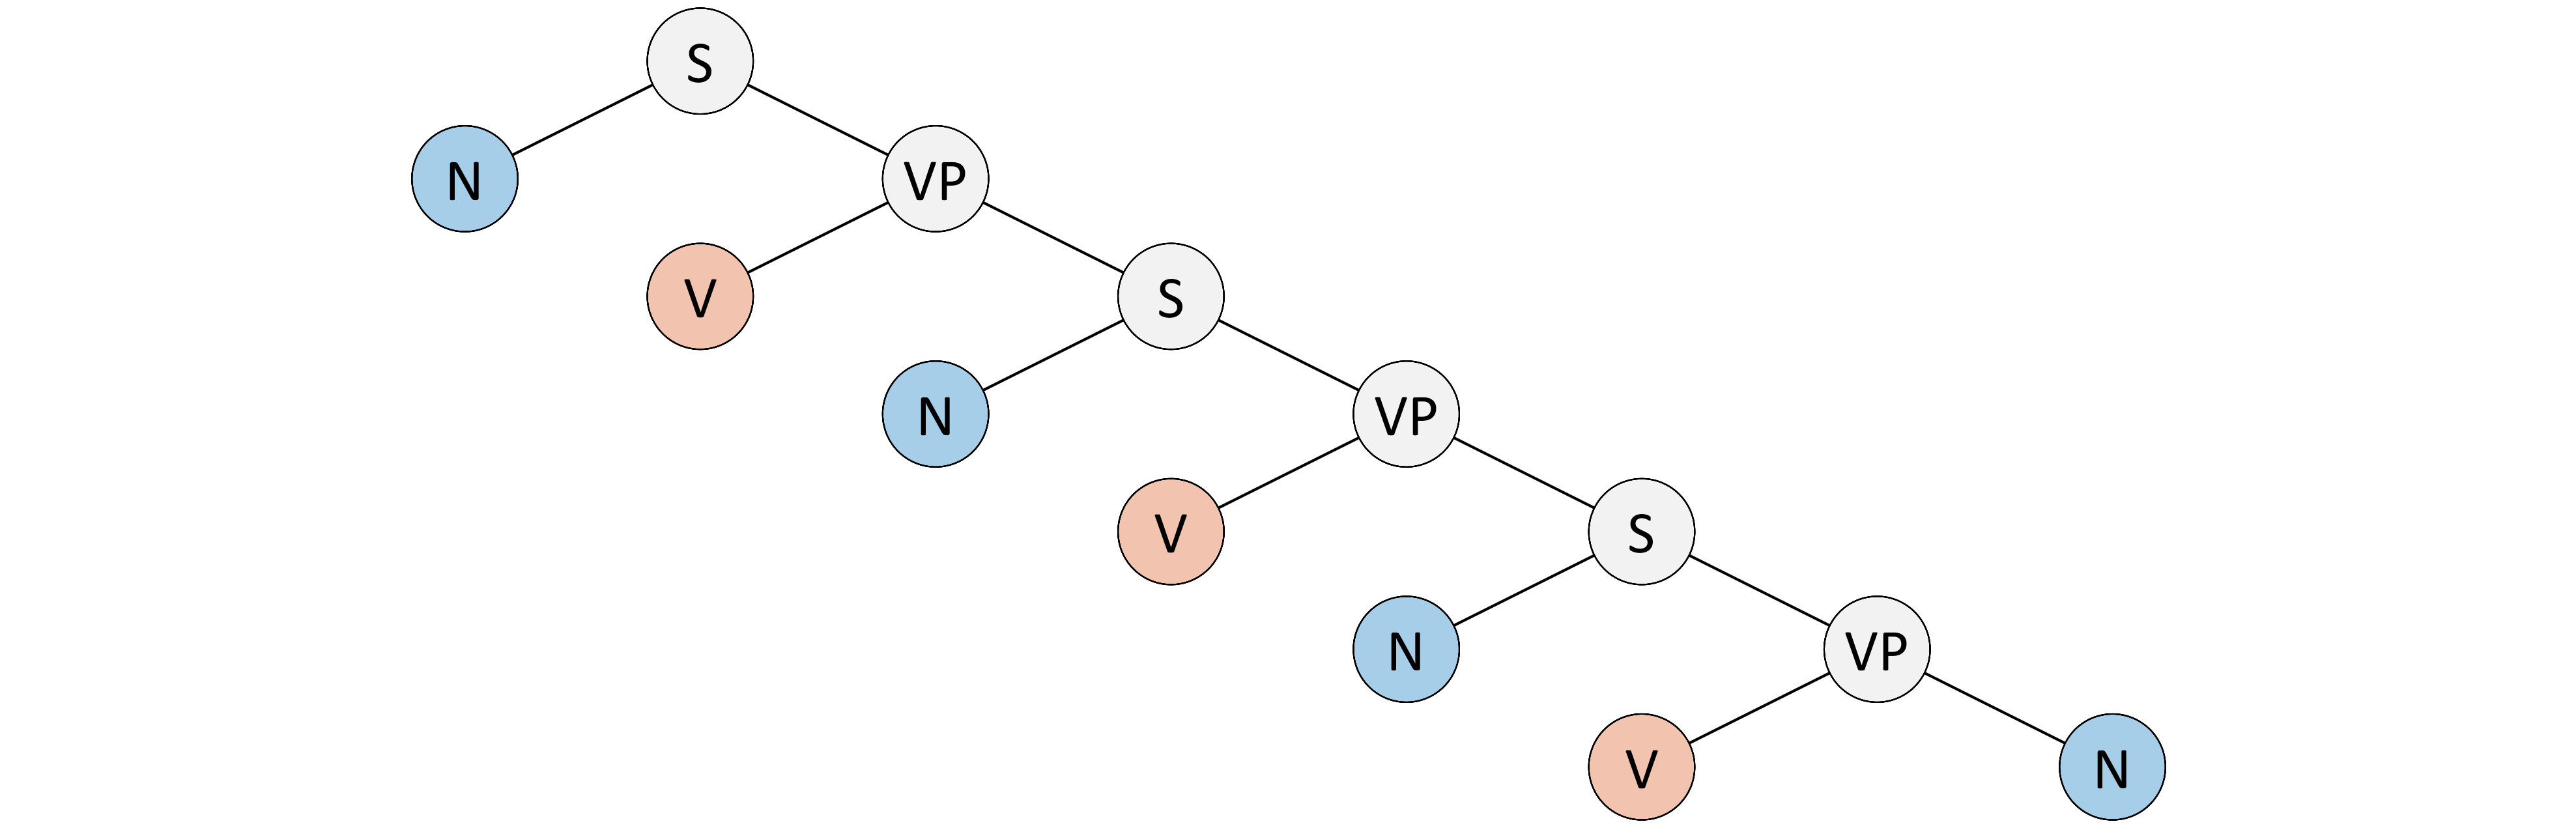
\includegraphics[width=\textwidth]{figures/Tilsen-img7.png}
\caption{The multiplicity problem: the same type of object can occur in multiple places in a structure.}
\label{fig:1:7}
\end{figure}
 

  The acceptance of multiplicity is so deeply ingrained (perhaps due to written language) that most theories fail to recognize the problem. The crux of the issue is that if we believe syntactic patterns can be understood in relation to macroscopic brain states, then we must accept a finite capacity for distinct states. A theory that allows for a multiplicitous conception of structure can provide no intrinsic mechanisms for understanding the nature of limitations on this capacity. Such limitations must be imposed extrinsically, in a manner that does not derive from the conception of structure which underlies the theory.

  Any syntactic theory must either ignore or resolve the \isi{multiplicity problem}. We should prefer a theory in which the resolution derives from the same conceptual model that provides a basis for a general understanding of linguistic phenomena—a \textit{comprehensive} theory. Many current approaches fall short of this because their solution is to distinguish between competence and performance, in effect stipulating that mechanisms of syntactic organization can be isolated from other cognitive mechanisms. The o/el framework addresses the \isi{multiplicity problem} by developing a mechanism for systems (construed microscopically as neural populations) to differentiate into subsystems (overlapping subpopulations). Because differentiated subsystems interfere with one another, differentiation leads to \isi{interference} that can destabilize those systems. Stability has important consequences for what speakers produce and what is coherent for an \isi{interpreter}.

  This book is organized into several chapters. The first chapter, \textsc{Overview of the oscillators/energy levels framework}, introduces the basic microscopic and macroscopic conceptual models which provide a basis for reasoning about syntactic phenomena. \textsc{Deconstructing syntactic theory} discusses how conventional syntactic theories are based on a small set of fundamental metaphors and image schemas, and contrasts these with the metaphors used in the oscillators/energy levels framework. \textsc{Reconstructing syntactic theory} provides a detailed presentation of the o/el model. The focus is on \isi{phrase structure}, but some \isi{morphosyntactic} and morphophonological phenomena are covered as well. Most importantly, the concept of \isi{interference} is developed in detail, and this motivates analyses in subsequent chapters. \textsc{Infinity and recursion} argues that viewing language as a discrete \isi{infinity} generated by recursive merge operations is misguided. \textsc{\isi{Grammaticality} intuitions} argues for reconceptualizing \isi{grammaticality} intuitions as the result of an experience of the \isi{coherence} of a system state trajectory; common neurophysiological patterns are interpreted in relation to \isi{coherence}. \textsc{Syntactic phenomena} applies the o/el framework to three phenomena: \isi{ellipsis}, \isi{anaphora}, and movement islands. Finally, \textsc{The \isi{physical linguistics} program} describes the philosophical underpinnings of the approach taken in this book, and sets the stage for future research.

  There is a small amount of mathematical formalization in this book, which will be of varying degrees of difficulty for readers, depending on their familiarity with dynamical systems. In most of the cases where equations are presented, I have provided illustrations which facilitate a visual conceptualization. It is my belief that a sufficient understanding of the mathematical concepts can be obtained from the visual/geometric illustrations alone, without a need for interpreting the symbolic math. The equations are merely a convenient shortcut for describing geometric patterns. For readers who would like to become more familiar with the relevant math, including how it can be related to behavior, I recommend two introductory texts: \textit{Dynamic Patterns: The self-organization of brain and behavior}, by J. A. Scott Kelso \citep{Kelso1997}, and \textit{Nonlinear dynamics and chaos}, by Steven H. Strogatz \citep{Strogatz2018}. Familiarity with these texts is not a prerequisite for understanding the current approach, but will undoubtedly enrich the interpretation. For more technical texts which address dynamics from biological, neurological, and physical perspectives, it is suggested that the reader consult \textit{The Geometry of Biological Time} by Arthur T. Winfree \citep{Winfree2001}, \textit{Dynamical Systems in Neuroscience} by Eugene M. Izhikevich \citep{Izhikevich2007}, and \textit{Advanced \isi{Synergetics}: Instability Hierarchies of Self-Organizing Systems and Devices} by Hermann \isi{Haken} \citep{Haken1983a}.

  Some portions of this book present critiques of “conventional” syntactic theories, especially in the second chapter, \textsc{Deconstructing syntactic theory,} and in the fourth chapter, \textsc{Infinity and recursion}. These critiques are related to the problems of \isi{atemporality} and multiplicity discussed above. A warning is necessary regarding the targets of the critiques. There are numerous syntactic theories/frameworks: 
  Minimalism \citep{Chomsky1995}, 
  Categorial Grammars (\citealt{Steedman1993,Wood2014}), 
  Tree Adjunction Grammars \citep{Joshi1987}, 
  Lexical Functional Grammar \citep{BresnanKaplan1982}, 
  Dependency Grammar (\citealt{Hudson1977,Tesnière2018}), 
  Generalized Phrase Structure Grammar 
  \citep{GazdarEtAl1985},
  Functional Grammar \citep{Dik1981}, 
  Role and reference grammar \citep{VanValinJr2014},
  Construction Grammar \citep{Goldberg1995}, 
  Radical Construction Grammar \citep{Croft2001}, 
  Sign-Based Construction Grammar \citep{Sag2012}, 
  Semiotic Grammar \citep{Mcgregor1997}, 
  Cognitive Grammar \citep{Langacker2008}, and others. It is beyond the scope of this book— %\todo{check dashes across document} 
  perhaps any single book—to critique all of these frameworks.

Rather than being general, the critiques herein specifically target Minimalism and its precursors, Transformational Grammar \citep{Chomsky1965} and Government and Binding Theory \citep{Chomsky1982}, which fall under the label of \isi{generative grammar}. These frameworks are the ones that we subsequently refer to as “conventional theories,” although this label is not intended to imply that these particular frameworks are more standard or widely accepted than others. Instead, “conventional” implicates a set of foundational metaphors which \textit{by convention} constitute a basis for reasoning about syntactic phenomena. However, narrowing the target of my critiques in this way raises the question of whether the critiques apply to other theories/frameworks. Certainly not all aspects of the critiques necessarily apply to all extant theories. It is left as a project for readers—many of whom are better versed in some of the particular approaches listed above—to consider whether the \isi{atemporality} and multiplicity problems (and the collections of critiques they encompass) apply to a given syntactic framework. Nonetheless, it is my impression as an outsider that the foundational metaphors discussed herein are very general, and I bring attention to the metaphors in order to provoke a re-examination of their usefulness.

